\documentclass{article}
\usepackage{tikz}
\usetikzlibrary{arrows.meta,positioning,calc,shapes.geometric}
\pagestyle{empty}
\begin{document}
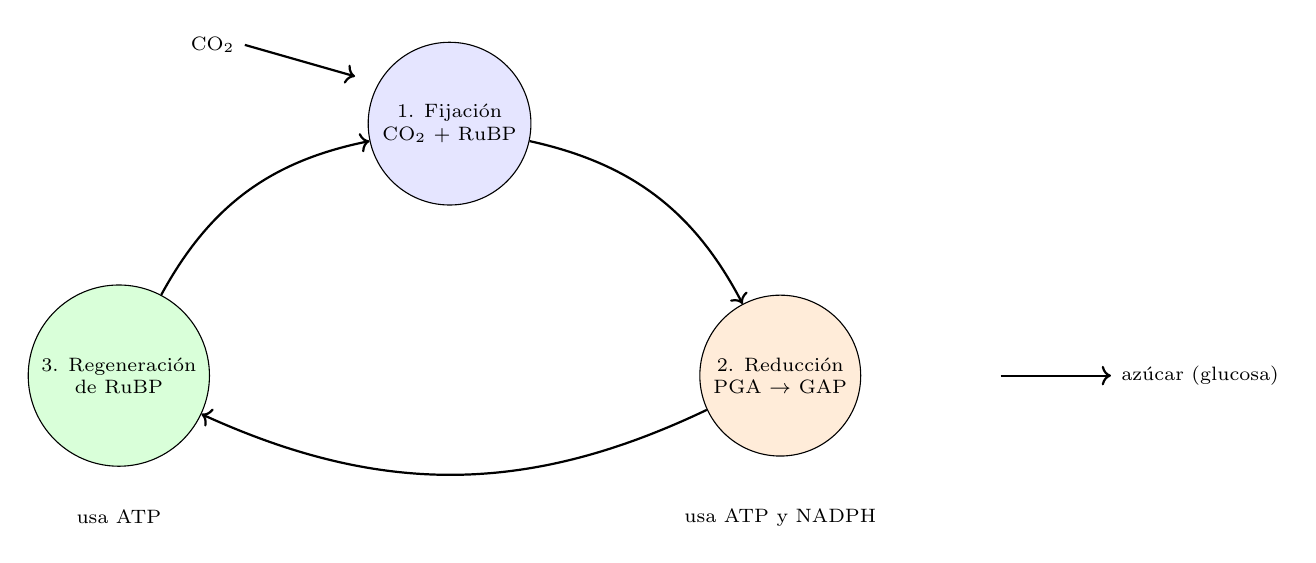
\begin{tikzpicture}
\tikzset{every node/.append style={align=center}}

\node[draw, circle, fill=blue!10, minimum size=2.0cm, align=center, font=\scriptsize] (a) at (0,2.2) {1. Fijación\\ CO$_2$ + RuBP};
\node[draw, circle, fill=orange!15, minimum size=2.0cm, align=center, font=\scriptsize] (b) at (4.2,-1.0) {2. Reducción\\ PGA $\to$ GAP};
\node[draw, circle, fill=green!15, minimum size=2.0cm, align=center, font=\scriptsize] (c) at (-4.2,-1.0) {3. Regeneración\\ de RuBP};
\draw[->, thick] (a) to[bend left=25] (b); \draw[->, thick] (b) to[bend left=25] (c); \draw[->, thick] (c) to[bend left=25] (a);
\node[font=\scriptsize, align=center] at (4.2,-2.8) {usa ATP y NADPH}; \node[font=\scriptsize, align=center] at (-4.2,-2.8) {usa ATP};
\draw[->, thick] (7.0,-1.0) -- (8.4,-1.0) node[right, font=\scriptsize] {azúcar (glucosa)}; \draw[->, thick] (-2.6,3.2) -- (-1.2,2.8) node[at start, left, font=\scriptsize] {CO$_2$};

\end{tikzpicture}
\end{document}
